% filename: chap-methodology-revised.tex
\chapter{Methodology and Implementation}
\label{chap:methodology}

Chapter~\ref{chap:problem} defined the formal CMDP governing telecom tower
energy management.  This chapter presents the implemented solution framework, including the
simulator, reinforcement-learning agent, safety mechanisms, training pipeline,
comparison policies, and evaluation protocol.  Practical simplifications relative to the formal model are
consolidated in Section~\ref{sec:impl_deviations}.


% ============================================================
\section{Methodology Overview}
\label{sec:overview}
% ============================================================

Figure~\ref{fig:workflow} shows the overall pipeline from raw data to
operational metrics.  The ITU/Zindi dataset is loaded and split per site into
a 45-day training block and a 15-day test block.  Each site's time series
drives a Gymnasium-compatible \texttt{TelecomEnv} simulator.  \texttt{MaskablePPO}
agents are trained within this simulator, producing a learned policy that is
subsequently frozen and evaluated across all ten sites under two logistics
scenarios.  Operational metrics---primarily Expected Energy Not Served
(EENS)---are computed from the evaluation rollouts.  Exploratory data analysis
of the dataset is presented in Chapter~\ref{chap:datasets-setup}.

\begin{figure}[htbp]
\centering
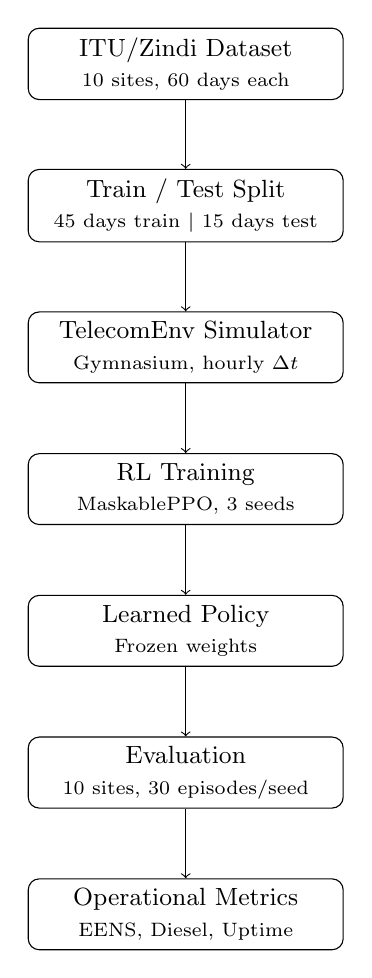
\begin{tikzpicture}[
  node distance=1.8cm,
  box/.style={draw, rounded corners, align=center,
              minimum width=4.0cm, minimum height=0.9cm, font=\small}
]
\node[box] (data)    {ITU/Zindi Dataset\\{\scriptsize 10 sites, 60 days each}};
\node[box, below of=data]   (split)   {Train / Test Split\\{\scriptsize 45 days train \textbar\ 15 days test}};
\node[box, below of=split]  (env)     {TelecomEnv Simulator\\{\scriptsize Gymnasium, hourly $\Delta t$}};
\node[box, below of=env]    (train)   {RL Training\\{\scriptsize MaskablePPO, 3 seeds}};
\node[box, below of=train]  (policy)  {Learned Policy\\{\scriptsize Frozen weights}};
\node[box, below of=policy] (eval)    {Evaluation\\{\scriptsize 10 sites, 30 episodes/seed}};
\node[box, below of=eval]   (metrics) {Operational Metrics\\{\scriptsize EENS, Diesel, Uptime}};

\draw[->] (data)    -- (split);
\draw[->] (split)   -- (env);
\draw[->] (env)     -- (train);
\draw[->] (train)   -- (policy);
\draw[->] (policy)  -- (eval);
\draw[->] (eval)    -- (metrics);
\end{tikzpicture}
\caption{End-to-end workflow of the proposed reinforcement-learning framework,
from dataset ingestion through policy training to operational evaluation.}
\label{fig:workflow}
\end{figure}


% ============================================================
\section{Rationale for the Proposed Methodology}
\label{sec:rationale}
% ============================================================

\subsection{Why PPO rather than value-based methods?}

The decision problem combines generator commitment and diesel ordering over
long horizons (720-step episodes).  Value-based methods such as DQN enumerate
$Q$-values for each action combination and are known to exhibit instability in
long-horizon environments with stochastic dynamics~\citep{mnih2015humanlevel}.
Proximal Policy Optimisation (PPO) optimises a parameterised policy directly
using a clipped surrogate objective that constrains update
magnitude~\citep{schulman2017proximal}, providing the training stability
required here.  PPO has demonstrated robust performance in long-horizon
control problems and energy-management
applications~\citep{perera2021application,zhang2021deep}, making it the
natural algorithm family for this work.

\subsection{Why MaskablePPO rather than penalty-based constraint handling?}

Penalty-based constraint handling adds infeasibility costs to the reward.
A finite penalty cannot guarantee zero hard violations: if the coefficient is
poorly calibrated the policy still explores infeasible actions, and a diesel
stockout or battery deep-discharge causes immediate, irreversible service loss.
\texttt{MaskablePPO} from \texttt{sb3-contrib} instead sets infeasible action
logits to $-\infty$ before the softmax, making the probability of any
infeasible action exactly zero by construction.  This converts the constraint
set $\mathcal{C}(s_t)$ into a hard structural property of the policy
distribution and eliminates penalty-coefficient tuning entirely.

\subsection{Why a unified agent (RLInv) alongside hierarchical decomposition
(TrackB)?}

Classical decomposed approaches use separate controllers for inventory
ordering and energy dispatch.  This ignores the bidirectional coupling: the
dispatch controller depletes inventory, while inventory level constrains which
dispatch actions are feasible.  A unified agent can in principle exploit this
coupling by jointly optimising both decisions from a single reward signal.
Whether that benefit justifies the added learning complexity is the central
empirical question (hypothesis H1).  Both architectures are therefore trained
and evaluated under identical conditions; neither outcome is assumed in advance.

\subsection{Why a discrete action space?}

Although battery dispatch could be formulated as a continuous RL action,
rural charge-controllers follow fixed priority rules rather than
continuous analogue setpoints.  The implemented system therefore delegates
battery dispatch to a deterministic priority rule, focusing RL learning
capacity on the logistics decisions (generator commitment and ordering)
where non-myopic planning is most valuable.

\subsection{Why a flat MLP rather than modular encoders?}

With a 9-dimensional observation vector, a two-layer flat MLP $[256,\,256]$
provides sufficient representational capacity.  Modular domain-specific
encoders introduce additional architectural hyperparameters (encoder depth,
output dimension, concatenation structure) with no demonstrated benefit at
this input dimensionality.  The flat design simplifies implementation and is
directly supported by the Stable-Baselines3 \texttt{MlpPolicy} without
a custom feature extractor.


% ============================================================
\section{Implemented Environment and Training Setup}
\label{sec:telecom_env}
% ============================================================

\subsection{Environment structure and observation}

The environment is implemented as a Gymnasium-compatible class
\texttt{TelecomEnv} operating at hourly resolution ($\Delta t = 1$\,h) with
720-step episodes (30 simulated days).  During training, a random start index
is sampled within the 45-day training block; evaluation is fixed to the
15-day test block.  Episodes terminate after 720 steps; no early termination
condition is used.

The 9-dimensional observation at each step is:
\begin{multline}
s_t = \bigl[
  \SoC_t,\;
  \Inv_t,\;
  \texttt{pending\_flag}_t,\;
  \texttt{pending\_qty}_t,\;
  P_t^{\PV},\; \\
  P_t^{\Load},\;
  G_t,\;
  \sin(2\pi h_t/24),\;
  \cos(2\pi h_t/24)
\bigr].
\end{multline}
The pending-delivery state uses a binary flag (order in transit?) and a
scalar quantity (fuel expected on arrival), which together are logically
equivalent to the single pipeline scalar $\Pipe_t$ of
Chapter~\ref{chap:problem} under the single-outstanding-order constraint.
Hour-of-day is encoded as sine--cosine features so that hours~23 and~0 are
adjacent in feature space.  Grid availability $G_t$ is treated as an
exogenous stochastic signal derived from the site time series rather than
a decision variable.  All continuous features are normalised online
using \texttt{VecNormalize}; statistics are frozen before evaluation.

\subsection{Action space, battery rule, and inventory}

The action space is discrete with six elements encoding
$\DG_t \in \{0,1\}$ and $Q_t \in \{0,\;0.30\,C^{\Tank},\;0.60\,C^{\Tank}\}$.
Battery dispatch is not a learnable action; it is determined by a fixed
energy-priority rule inside the simulator:
\[
\text{PV} \;\to\; \text{Grid} \;\to\; \text{Battery discharge}
\;\to\; \text{DG} \;\to\; \text{Unmet load.}
\]

Diesel inventory is tracked in kWh-equivalent units.  Tank capacity is
$C^{\Tank} = 72\,\bar{D}$ (approximately three days of full-load backup,
where $\bar{D}$ is the site mean hourly load).  A generator start is
permitted only if
$\Inv_t \geq 1.20 \times P_{\mathrm{rated}}^{\DG} \times 2\,\mathrm{h}$,
ensuring sufficient fuel for at least two hours of operation with a 20\% safety margin.  Diesel delivery delay is modelled as
a geometric process: once an order is placed, delivery occurs at each
subsequent step with probability $p_{\text{normal}}=1/24$ (mean 24\,h,
normal scenario) or $p_{\text{delayed}}=1/48$ (mean 48\,h, delayed
scenario).  The geometric model preserves a Markovian state with only the
two pending-order scalars, avoiding a countdown vector.

\subsection{Safety handling}

Safety is enforced through hard action masking applied at every step.
Two rules are checked before the policy samples an action.

\begin{enumerate}
  \item \textbf{DG masking:} all actions with $\DG_t = 1$ are disabled if
  inventory is below the minimum startup threshold, preventing forced
  mid-run shutdowns.
  \item \textbf{Order masking:} all non-zero order actions are disabled if
  a delivery is already pending, enforcing the single-outstanding-order
  constraint.  Order quantities exceeding remaining tank headroom are also
  clipped.
\end{enumerate}

\texttt{MaskablePPO} applies the mask by setting infeasible logits to
$-\infty$ before the softmax; the no-operation action is always feasible
as a safe fallback.  Post-step physical clipping (SoC and inventory to
their bounds) provides a numerical backstop and contributes a small
penalty $\mu V_t$ to the reward.  No adaptive Lagrangian update was
implemented; masking alone drove hard violations to zero across all
evaluated conditions.

\subsection{Reward function}

The reward is a shaped, normalised scalar designed to penalise unreliability
far more heavily than fuel cost:
\[
r_t =
-\alpha \dfrac{E_t^{\DG}}{\bar{D}}
-\beta  \dfrac{E_t^{\Grid}}{\bar{D}}
-\lambda \dfrac{U_t}{\bar{D}}
-\gamma_r\,\mathbb{I}\!\bigl[U_t>0 \wedge \Inv_t=0\bigr]
-\mu\,V_t,
\]
where $E_t^{\DG}$ is diesel energy consumed, $E_t^{\Grid}$ is grid energy
drawn, $U_t$ is unmet load energy (kWh), $\mathbb{I}[\cdot]$ is a cliff penalty
triggered by a stockout coinciding with an active load shortfall, and
$V_t$ indicates a physical-clipping event.  The default coefficients are
$\alpha=1.0$, $\beta=0.4$, $\lambda=100$, $\gamma_r=200$, $\mu=20$.
This formulation prioritises service reliability over fuel efficiency,
ensuring the learned policy strongly avoids stockouts and unmet load events
even at the cost of higher diesel consumption.  Dividing all energy terms
by $\bar{D}$ normalises the signal to a comparable scale across sites.
The implemented reward is a shaped approximation of the economic cost
objective defined in Chapter~\ref{chap:problem}; monetary cost components
such as ordering cost, holding cost, and carbon cost are not explicitly
represented.

\subsection{Agent architecture and training}

RLInv uses \texttt{MaskablePPO} with a flat MLP $[256,\,256]$ policy.
Training used four parallel \texttt{SubprocVecEnv} environments for
400{,}000 timesteps per seed across three seeds (42, 123, 777).  Three
independent seeds were used to quantify training variability while remaining
feasible under the available CPU training budget.  A custom
evaluation callback synchronised \texttt{VecNormalize} statistics between
the training and evaluation environments before each validation pass,
preventing observation-scale mismatch.  Training inventory was fixed at
$0.6\,C^{\Tank}$ to reduce early-episode variance; evaluation randomises
initial inventory over $[0.3,\,0.9]\,C^{\Tank}$.

A convergence check extended training to 560{,}000 steps on three
representative sites (1, 5, and~7) using seed~42.  Sites~1 and~7
showed no change in evaluation reward beyond 400{,}000 steps,
indicating early convergence.  Site~5 exhibited high reward
variance across independent runs regardless of step count,
consistent with its classification as a grid-constrained site.
The 400{,}000-step checkpoint was therefore retained for all sites.

Table~\ref{tab:hyperparams} lists all hyperparameters.

\begin{table}[htb]
\centering
\small
\caption{Training hyperparameters for RLInv and the TrackB dispatch agent.}
\label{tab:hyperparams}
\begin{tabular}{p{3.8cm}p{4.2cm}p{5.0cm}}
\toprule
\textbf{Parameter} & \textbf{Value} & \textbf{Rationale} \\
\midrule
Algorithm              & MaskablePPO (\texttt{sb3-contrib}) & Hard feasibility masking \\
Policy network         & Flat MLP [256,\,256], ReLU         & CPU-feasible capacity \\
Total timesteps        & 400{,}000 per seed                 & $\approx$\,2\,h on a 6--8 core CPU workstation \\
Learning rate          & $3\times10^{-4}$ (linear decay)    & PPO standard \\
Clip ratio $\epsilon$  & 0.2                                & PPO standard \\
Entropy coefficient    & 0.01                               & Encourage exploration \\
Discount $\gamma$      & 0.99                               & Effective horizon $\approx$\,100\,h covers typical delivery lead times while reducing return variance \\
GAE $\lambda$          & 0.95                               & Bias--variance balance \\
$n_{\text{steps}}$     & 2048                               & Rollout buffer length \\
Batch size             & 256                                & CPU-friendly mini-batch \\
$n_{\text{epochs}}$    & 10                                 & PPO inner loop \\
Parallel environments  & 4 (\texttt{SubprocVecEnv})         & CPU parallelism; reduced from 8 due to OS process handle limits \\
Seeds                  & 42, 123, 777                       & Mean $\pm$ std reported \\
\bottomrule
\end{tabular}
\end{table}


% ============================================================
\section{Comparison Policies}
\label{sec:comparison_policies}
% ============================================================

Six policies are evaluated.  The two principal architectures, RLInv and
TrackB, differ fundamentally in how they couple the ordering and dispatch
decisions; Figure~\ref{fig:rlinv_trackb} illustrates this structural
contrast.

\begin{figure}[htbp]
\centering
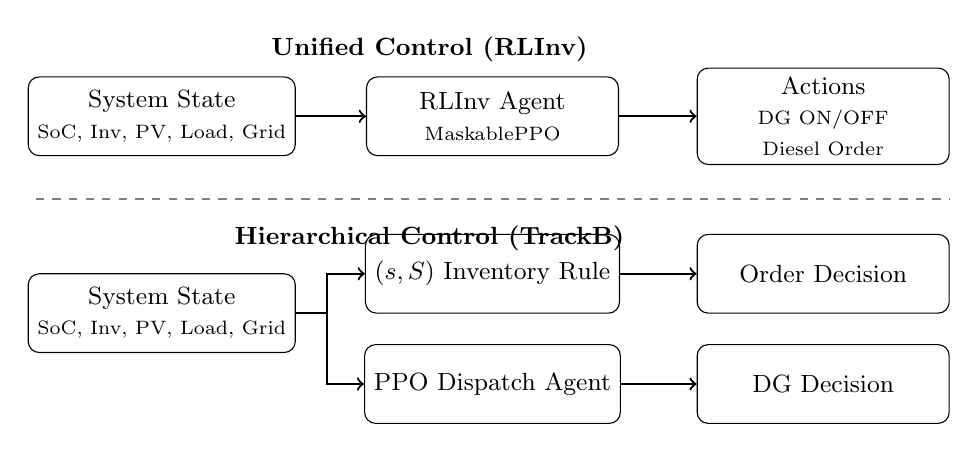
\begin{tikzpicture}[
  box/.style={draw, rounded corners=4pt, align=center,
              minimum width=3.2cm, minimum height=1.0cm, font=\small},
  arrow/.style={->, thick},
  label/.style={font=\small\bfseries}
]
%% ---- RLInv row (y = 0) ----
\node[label] at (3.4, 0.85) {Unified Control (RLInv)};
\node[box] (state1) at (0, 0)
  {System State\\{\scriptsize SoC, Inv, PV, Load, Grid}};
\node[box] (agent1) at (4.2, 0)
  {RLInv Agent\\{\scriptsize MaskablePPO}};
\node[box] (acts1) at (8.4, 0)
  {Actions\\{\scriptsize DG ON/OFF}\\{\scriptsize Diesel Order}};
\draw[arrow] (state1) -- (agent1);
\draw[arrow] (agent1) -- (acts1);
%% ---- dividing rule ----
\draw[dashed, gray] (-1.6, -1.05) -- (10.0, -1.05);

%% ---- TrackB rows ----
\node[label] at (3.4, -1.55) {Hierarchical Control (TrackB)};

\node[box] (state2) at (0, -2.5)
  {System State\\{\scriptsize SoC, Inv, PV, Load, Grid}};

\node[box] (ss)       at (4.2, -2.0) {$(s,S)$ Inventory Rule};
\node[box] (order2)   at (8.4, -2.0) {Order Decision};

\node[box] (dispatch) at (4.2, -3.4) {PPO Dispatch Agent};
\node[box] (dg2)      at (8.4, -3.4) {DG Decision};

\draw[arrow] (state2.east) -- ++(0.4,0) |- (ss.west);
\draw[arrow] (state2.east) -- ++(0.4,0) |- (dispatch.west);
\draw[arrow] (ss)       -- (order2);
\draw[arrow] (dispatch) -- (dg2);

\end{tikzpicture}
\caption{Structural comparison of the two control architectures. RLInv
jointly optimises generator dispatch and diesel ordering within a single
reinforcement-learning policy. TrackB separates the two decisions: a
classical $(s,S)$ rule handles ordering while a PPO agent handles dispatch.
The experiment tests whether joint optimisation (RLInv) delivers a
measurable reliability improvement over hierarchical decomposition (TrackB).
Ablation A6 (not shown) uses the same hierarchical ordering structure as
TrackB but replaces the dispatch controller with an RL policy operating
over a reduced \texttt{Discrete(2)} action space.}
\label{fig:rlinv_trackb}
\end{figure}

\textbf{RLInv} is the proposed unified controller: \texttt{MaskablePPO}
learns to select generator commitment and diesel order quantity jointly at
each step, with all three masking rules active.

\textbf{TrackB} is the hierarchical comparison: a calibrated $(s,S)$
inventory rule determines ordering (reorder point = mean daily consumption
$\times$ mean lead time $+$ 48-h safety buffer; order-up-to level =
$0.85\,C^{\Tank}$), while a PPO dispatch agent with the same MLP
architecture as RLInv controls the generator.  Using an identical network
ensures that performance differences reflect control structure rather than
network capacity.

\textbf{B0} is a rule-based heuristic: threshold dispatch with fixed-interval
ordering, requiring no training.  \textbf{B1} replaces fixed ordering in B0
with the calibrated $(s,S)$ rule.  \textbf{A7} is vanilla PPO trained without
action masking, isolating the contribution of the safety mechanism; it is
evaluated primarily on sites exhibiting non-trivial reliability challenges,
where constraint violations are most likely to occur.
\textbf{A5} is RLInv with inventory observations zeroed via a
\texttt{NoInvObsWrapper}, isolating the contribution of explicit inventory
awareness in the state.

\textbf{A6} isolates the contribution of the learned ordering policy.
In this variant the RL agent controls only generator commitment under a
reduced \texttt{Discrete(2)} action space, while diesel ordering is handled
by the same calibrated $(s,S)$ rule used in TrackB.  The observation space,
reward function, and environment dynamics remain identical to RLInv.
Because the dispatch policy is re-learned under the smaller action space,
A6 provides a cleaner ordering ablation than TrackB, although the comparison
is not perfectly controlled.

Table~\ref{tab:ablation-design} maps every policy to the hypothesis it tests.
The B0\,$\to$\,B1\,$\to$\,TrackB\,$\to$\,RLInv ladder isolates the contribution
of each architectural layer in turn: intelligent ordering, learned dispatch,
and joint co-optimisation.  Ablation A6 complements this ladder by holding
dispatch architecture constant while substituting classical ordering,
providing a cleaner test of the ordering contribution than TrackB alone.

\begin{table}[htb]
\centering
\small
\caption{Policies evaluated in the experimental campaign and the hypothesis
each tests.}
\label{tab:ablation-design}
\begin{tabular}{p{1.8cm}p{7.5cm}p{3.5cm}}
\toprule
\textbf{Label} & \textbf{Description} & \textbf{Hypothesis} \\
\midrule
B0      & Threshold dispatch, fixed-interval ordering            & Baseline anchor \\
B1      & Threshold dispatch, $(s,S)$ ordering                  & Ordering value (H1) \\
A7      & Vanilla PPO, no action masking                        & Safety mechanisms (H2) \\
TrackB  & $(s,S)$ ordering $+$ PPO dispatch                    & Decomposition vs.\ joint (H1) \\
A5      & RLInv, inventory observations zeroed                  & Inventory state value (H3) \\
A6      & RLInv dispatch only (\texttt{Discrete(2)}) $+$ $(s,S)$ ordering & Ordering value, cleaner H1 test \\
RLInv   & Full proposed system                                  & Reference \\
\bottomrule
\end{tabular}
\end{table}


% ============================================================
\section{Evaluation Protocol}
\label{sec:evaluation_protocol}
% ============================================================

All policies are evaluated on the 15-day test window (days~46--60) of each
of the ten ITU/Zindi sites, with 30 episodes per seed and initial inventory
randomised uniformly over $[0.3,\,0.9]\,C^{\Tank}$.  RLInv, TrackB, and A6
are evaluated under both the normal ($p=1/24$) and delayed ($p=1/48$)
logistics scenarios to enable direct cross-scenario comparison.  Baselines
and the remaining ablations are evaluated under the normal scenario only.

The primary metric is EENS (kWh per 30-day episode).  Sites with mean EENS
exceeding 50\,kWh under at least one policy are classified as
\emph{constrained} and receive focused statistical analysis; below this
threshold all policies achieve near-zero EENS and cannot be meaningfully
discriminated.  RLInv, TrackB, and A6 are evaluated under both the normal
and delayed logistics scenarios to enable direct cross-scenario comparison;
baselines and remaining ablations are evaluated under the normal scenario only.
Statistical comparisons use seed-level means ($n=3$) as the
unit of analysis; Welch's $t$-tests and Cohen's $d$ are reported alongside
$p$-values to account for the small sample size.


% ============================================================
\section{Implementation Deviations from the Formal Model}
\label{sec:impl_deviations}
% ============================================================

Although the implementation follows the CMDP formulation of
Chapter~\ref{chap:problem} closely, several practical simplifications were
adopted to enable stable training within the available CPU budget.
Table~\ref{tab:deviations} consolidates these points; each deviation was adopted for a
specific practical reason and does not invalidate the empirical study, but
defines the scope within which results should be interpreted.

\begin{table}[htb]
\centering
\small
\caption{Deviations between the formal CMDP (Chapter~3) and the implemented
system.}
\label{tab:deviations}
\begin{tabular}{p{2.8cm}p{4.6cm}p{4.6cm}}
\toprule
\textbf{Aspect} & \textbf{Formal model} & \textbf{Implementation} \\
\midrule
Battery control
  & $P_t^{\Bat}$ included in CMDP action space (Chapter~3)
  & Fixed energy-priority rule; not an RL decision \\[4pt]
Action space
  & Hybrid continuous $+$ discrete
  & Discrete 6-action encoding \\[4pt]
Lead-time model
  & Lognormal($\mu$\,=\,2.5\,days normal; 5.0\,days delayed), single scalar $\Pipe_t$
  & Geometric distribution ($p$\,=\,1/24, mean 24\,h normal; $p$\,=\,1/48, mean 48\,h
    delayed); flag\,+\,quantity pair. Shorter mean delays maintain adequate
    training signal within the 30-day episode horizon. \\[4pt]
Discount factor
  & $\gamma = 0.995$ (effective horizon $\approx$\,200\,h)
  & $\gamma = 0.99$ (SB3 default; effective horizon $\approx$\,100\,h
    covers typical delivery lead times while reducing
    return variance during training) \\[4pt]
Reward
  & Economic cost decomposition (monetary)
  & Shaped normalised scalar \\[4pt]
Safety mechanisms
  & Masking $+$ recovery $+$ Lagrangian
  & Masking $+$ physical clipping only \\[4pt]
Neural architecture
  & Modular domain-specific encoders
  & Flat MLP $[256,\,256]$, ReLU \\[4pt]
Training budget
  & 576{,}000 steps (script default)
  & 400{,}000 steps (final run); convergence check extended
    training to 560{,}000 steps confirming plateau \\
\bottomrule
\end{tabular}
\end{table}